\documentclass[aspectratio=169,10pt]{beamer}

\usepackage[utf8]{inputenc}
\usepackage[T1]{fontenc}
\usepackage[spanish]{babel}
\usepackage{booktabs}
\usepackage{graphicx}
\usepackage{tikz}
\usepackage{amsmath}
\usepackage{hyperref}
\usetikzlibrary{arrows.meta,positioning,shapes}

\usetheme{Madrid}
\definecolor{DARLblue}{RGB}{22,66,105}
\definecolor{DARLteal}{RGB}{28,132,137}
\definecolor{DARLgold}{RGB}{220,153,45}
\definecolor{DARLgray}{RGB}{80,88,96}
\setbeamercolor{structure}{fg=DARLblue}
\setbeamercolor{title}{fg=white,bg=DARLblue}
\setbeamercolor{frametitle}{fg=white,bg=DARLblue}
\setbeamercolor{block title}{fg=white,bg=DARLteal}
\setbeamercolor{block body}{fg=black,bg=black!4}
\setbeamertemplate{navigation symbols}{}
\setbeamertemplate{footline}[frame number]
\graphicspath{{kaggle/dqn-dummy/v4/outputs/figures/}}

\title[DARL DQN Dummy v4]{Comparación de utilidad y costo de las acciones\\y diagnóstico de estabilidad}
\subtitle{Informe metodológico de DARL DQN Dummy v4}
\author{Proyecto de tesis DARL}
\institute{Demostración experimental con datos PhysioNet y etiqueta sintética}
\date{Corrida auditada: v4, semilla 42}

\begin{document}

\begin{frame}
  \titlepage
\end{frame}

\begin{frame}{Resumen ejecutivo}
\begin{itemize}
  \item \textbf{v4 sí terminó de ejecutarse}, pero su estado es
        \texttt{needs\_improvement}: el acuerdo de acciones entre los dos
        últimos checkpoints fue \textbf{85\%}, menor que el umbral de 95\%.
  \item La variación del retorno de validación sí pasó: \textbf{1,47\%}
        frente al máximo permitido de 5\%.
  \item El agente entrenó los \textbf{1000 episodios} disponibles; aumentar
        episodios sin diagnosticar la causa no garantiza estabilidad.
  \item La comparación de políticas favorece acciones distintas según el tipo
        de cambio: A2 para covariate drift y A3 para concept drift.
  \item Los signos vitales son reales, pero el objetivo y los cambios de
        distribución son \textbf{sintéticos}. No es una validación clínica.
\end{itemize}
\vspace{0.3em}
\begin{block}{Lectura principal}
Retorno casi constante no implica que el agente repita las mismas acciones.
En v4, la puntuación agregada fue estable, pero la política aún cambiaba en
parte de las situaciones de validación.
\end{block}
\end{frame}

\begin{frame}{Ficha de datos y alcance}
\begin{columns}[T]
\column{0.52\textwidth}
\begin{block}{Datos}
\begin{itemize}
  \item Base: registros procesados de PhysioNet/Computing in Cardiology
        Challenge 2019 \cite{reyna2020sepsis}.
  \item 1\,552\,210 filas y 40\,336 pacientes en la corrida registrada.
  \item Entradas: HR, O2Sat, Temp, SBP, MAP, DBP y Resp.
  \item La etiqueta que aprende XGBoost es \texttt{y\_dummy}
        (prevalencia 46,7\%); \texttt{SepsisLabel} solo se usa para
        estratificar particiones.
\end{itemize}
\end{block}
\column{0.48\textwidth}
\begin{block}{Diseño de la demostración}
\begin{itemize}
  \item Partición por paciente: A para ajuste inicial; B para entrenamiento,
        validación y prueba.
  \item Replay: hasta 200 camas, 16 días simulados; 15 decisiones diarias por
        escenario y resultado evaluado al día siguiente.
  \item Escenarios: estable, covariate, concept y combinado.
  \item Corrida registrada: semilla 42; prueba de una sola semilla.
\end{itemize}
\end{block}
\end{columns}
\vspace{0.2em}
{\footnotesize \textcolor{DARLgray}{AUC reportada = ROC-AUC sobre la etiqueta
sintética. No representa sensibilidad clínica ni desempeño para diagnosticar
sepsis.}}
\end{frame}

\begin{frame}{Auditoría de los ocho CSV de v4}
\scriptsize
\begin{tabular}{p{0.23\textwidth}p{0.13\textwidth}p{0.55\textwidth}}
\toprule
\textbf{Archivo} & \textbf{Filas} & \textbf{Comprobación principal} \\
\midrule
\texttt{actions.csv} & 420 & 7 políticas \(\times\) 4 escenarios \(\times\) 15 acciones; cero fallbacks y cero diferencias entre solicitada y ejecutada. \\
\texttt{action\_audit.csv} & 60 & 4 \(\times\) 15 decisiones; utilidades completas y regret no negativo. \\
\texttt{calibration.csv} & 6 & 3 velocidades por tipo; covariate 0,25 y concept 0,15 son las velocidades más lentas que califican. \\
\texttt{daily\_metrics.csv} & 448 & 7 políticas \(\times\) 4 \(\times\) 16 días; AUC completa; 28 recompensas terminales vacías, una por trayectoria. \\
\texttt{drift\_dia1\_vs\_dia16.csv} & 2 & Resumen descriptivo solo para covariate y concept; no cubre stable ni combined. \\
\texttt{policy\_comparison.csv} & 28 & 7 políticas \(\times\) 4 escenarios; 15 recompensas válidas cada una, sin intervalos de incertidumbre. \\
\texttt{stage\_calendar.csv} & 64 & 4 calendarios completos de 16 días; covariate inicia día 5 y concept día 5 o 7 en combined. \\
\texttt{training\_history.csv} & 1000 & 100 checkpoints de validación, cada 10 episodios; campos vacíos en episodios sin validación son esperados. \\
\bottomrule
\end{tabular}
\vspace{0.2em}
{\tiny El manifiesto declara 18 rutas gráficas (9 PNG y 9 SVG); en el directorio
hay 17 PNG y ningún SVG. Las variantes 04a/b, 05a/b y 07a/b, más las figuras
10--11 del notebook auxiliar, requieren conservar su propia procedencia.}
\vspace{0.35em}
\begin{block}{Control de integridad}
Los conteos y las ausencias corresponden a la estructura del experimento; no
encontré filas duplicadas en la comparación política--escenario ni faltantes
en las utilidades de \texttt{action\_audit.csv}.
\end{block}
\end{frame}

\begin{frame}{Qué mide cada CSV y qué no permite concluir}
\begin{itemize}
  \item \texttt{policy\_comparison.csv}: compara cada política sobre el replay
        reservado. \texttt{mean\_auc} promedia los 16 días observados; el
        \texttt{return} suma 15 recompensas de acción al día siguiente.
  \item \texttt{action\_audit.csv}: compara las cuatro acciones desde el mismo
        pipeline del día y calcula regret inmediato. Es un oracle de un paso,
        no la política óptima para todo el horizonte.
  \item \texttt{calibration.csv}: selecciona velocidades con tres reglas
        predefinidas en B-train; no es una evaluación de generalización.
  \item \texttt{drift\_dia1\_vs\_dia16.csv}: el KS compara días con cohortes
        de pacientes distintas por el recambio del replay; describe el cambio
        total entre días, no aísla por sí solo el efecto causal de la inyección.
  \item La corrida usa una sola semilla. Las diferencias de retorno/AUC son
        observaciones de esta ejecución, no estimaciones con incertidumbre.
\end{itemize}
\end{frame}

\begin{frame}{Mapa del notebook v4: datos y entorno}
\footnotesize
\begin{tabular}{p{0.25\textwidth}p{0.68\textwidth}}
\toprule
\textbf{Sección / funciones} & \textbf{Qué hace y qué verificar} \\
\midrule
Configuración; \texttt{checkpoint} & Fija semilla, rutas, hiperparámetros, dispositivo y escribe \texttt{run\_summary.json}. \\
\texttt{find\_parquet} & Localiza el parquet y valida columnas, llave paciente--ICULOS y orden temporal. \\
\texttt{split\_ids}, \texttt{roles} & Divide por paciente y separa roles de actualización y evaluación. \\
\texttt{canonical\_scores}, \texttt{flip\_bit}, \texttt{concept\_weights}, \texttt{concept\_threshold} & Construye el objetivo sintético y las trayectorias de relación features--etiqueta. \\
\texttt{make\_replay} & Reproduce hasta 200 camas, 100 por rol, y recambia camas al agotar observaciones. \\
\texttt{Pipeline.act}, \texttt{auc}, \texttt{utility} & Implementa A1--A4, evalúa ROC-AUC y penaliza tiempo normalizado. \\
\texttt{ramp}, \texttt{inject} & Aplica covariate drift a vitales y concept drift a \texttt{y\_dummy}. \\
\bottomrule
\end{tabular}
\vspace{0.2em}
\begin{block}{Interpretación}
Esta primera mitad fabrica el mundo simulado. PhysioNet aporta los registros
de signos vitales; el resultado de aprendizaje y ambos cambios son artificiales.
\end{block}
\end{frame}

\begin{frame}{Mapa del notebook v4: señales, agente y evaluación}
\scriptsize
\begin{tabular}{p{0.27\textwidth}p{0.66\textwidth}}
\toprule
\textbf{Sección / funciones} & \textbf{Qué hace y qué verificar} \\
\midrule
\texttt{build\_reference}, \texttt{psi}, \texttt{monitor} & Define referencia por vital y calcula KS, PSI, AUC y saturación antes de actuar. \\
\texttt{encode\_observation} & Codifica KS, PSI y AUC en categorías; concatena el historial de tres días (estado de 30 entradas). \\
\texttt{BedEnv.reset}, \texttt{\_observe}, \texttt{step} & Entrega la observación, ejecuta la actualización y revela la AUC del día siguiente. \\
\texttt{QNetwork}, \texttt{ReplayBuffer}, \texttt{DQNAgent.learn} & Red 30--128--128--4; replay FIFO; objetivo Double DQN, Huber y copia target cada 50 actualizaciones. \\
\texttt{calibrate} & Elige las velocidades más lentas que cumplen umbrales de caída y recuperación en B-train. \\
\texttt{choose\_policy}, \texttt{roll} & Ejecuta DQN/baselines y, opcionalmente, evalúa el oracle inmediato desde el pipeline actual. \\
\texttt{agreement}, \texttt{train\_agent} & Valida cada 10 episodios, selecciona checkpoint por media móvil y calcula variación/acuerdo. \\
\texttt{make\_figures}, \texttt{run\_experiment} & Exporta gráficos, CSV y gates; persiste estado de ejecución. \\
\bottomrule
\end{tabular}
\vspace{0.2em}
\begin{block}{Punto de lectura crítica}
\texttt{positive\_dqn\_return} no es un gate informativo: la recompensa suma AUC
absoluta menos un costo pequeño, así que un retorno positivo es esperable
incluso sin aprender una política superior.
\end{block}
\end{frame}

\begin{frame}{Acciones y justificación de la comparación}
\small
\setlength{\tabcolsep}{3pt}
\begin{tabular}{p{0.11\textwidth}p{0.35\textwidth}p{0.46\textwidth}}
\toprule
\textbf{Acción} & \textbf{Intervención} & \textbf{Papel experimental} \\
\midrule
A1 & No actualizar el pipeline. & Control de costo mínimo: muestra cuánto
se degrada el modelo sin mantenimiento. \\
A2 & Recalibrar mediana/IQR y clipping; conservar XGBoost. &
Prueba una intervención sobre la representación, pertinente cuando cambia
\(P(X)\) y la relación predictiva se mantiene. \\
A3 & Reentrenar XGBoost; conservar el transformador actual. &
Prueba una intervención sobre el modelo, pertinente cuando cambia
\(P(Y\mid X)\). \\
A4 & Actualizar transformador y XGBoost. &
Referencia de actualización completa; no es el foco de la tabla, pero sirve
para normalizar el costo y contextualizar el máximo de intervención. \\
\bottomrule
\end{tabular}

\vspace{0.6em}
\begin{block}{Utilidad y costo}
\footnotesize
El DQN selecciona acciones discretas con una recompensa que penaliza el tiempo
de intervención. A1 es un control, A2 y A3 aíslan las dos etapas del pipeline,
y A4 permite contrastar el costo de una actualización completa. DQN se basa en
Q-learning con aproximación profunda; A1--A4 son intervenciones del diseño y no
implican que cada drift requiera una acción única
\cite{mnih2015dqn,chen2016xgboost}.
\end{block}
\end{frame}

\begin{frame}{Flujo propuesto de comparación}
\centering
\begin{tikzpicture}[
  scale=0.86,transform shape,
  node distance=0.35cm and 0.35cm,
  box/.style={draw=DARLblue,rounded corners,fill=DARLblue!6,
              align=center,text width=2.05cm,minimum height=1.0cm},
  process/.style={draw=DARLteal,rounded corners,fill=DARLteal!8,
                  align=center,text width=2.1cm,minimum height=1.0cm},
  arrow/.style={-{Latex[length=2mm]},thick,DARLgray}
]
\node[box] (data) {Datos\\PhysioNet +\\objetivo sintético};
\node[box,right=of data] (split) {Partición por\\paciente\\A / B-train / val / test};
\node[box,right=of split] (scenario) {Replay común\\4 escenarios\\de drift gradual};
\node[process,below=of scenario] (observe) {Observación diaria\\KS, PSI, AUC y\\historial reciente};
\node[process,left=of observe] (actions) {Política\\DQN o fija\\A1--A4};
\node[process,left=of actions] (score) {Evaluar día +1\\ROC-AUC, tiempo\\y costo};
\node[box,below=of actions] (compare) {Comparar retorno,\\costo y regret\\por escenario};
\node[box,below=of score] (check) {Validación\\convergencia del retorno\\y acuerdo de acciones};
\draw[arrow] (data)--(split);
\draw[arrow] (split)--(scenario);
\draw[arrow] (scenario)--(observe);
\draw[arrow] (observe)--(actions);
\draw[arrow] (actions)--(score);
\draw[arrow] (score)--(check);
\draw[arrow] (score)--(compare);
\draw[arrow] (actions)--(compare);
\end{tikzpicture}

\vspace{0.1em}
{\footnotesize \textbf{Regla de separación:} calibrar y seleccionar en B-train/B-val;
usar B-test solo para el reporte final. No reajustar hiperparámetros después
de mirar el resultado de prueba.}
\end{frame}

\begin{frame}{Definición de utilidad y costo}
\begin{equation*}
  r_t = \operatorname{ROC\!-\!AUC}_{t+1}
        - \lambda \frac{T(a_t)}{T_{\mathrm{ref}}},
  \qquad \lambda=0{,}05
\end{equation*}
\textbf{Donde:} \(r_t\) es la recompensa al evaluar el día posterior;
\(a_t\) es la acción tomada; \(T(a_t)\) es su tiempo medido; y
\(T_{\mathrm{ref}}\) es el tiempo de referencia de A4 usado para normalizar
el costo.

\vspace{0.3em}
\begin{itemize}
  \item El retorno de una política es la suma de recompensas válidas en los
        15 días evaluables; la media ROC-AUC se reporta aparte.
  \item Costo de acción normalizado observado en B-train:
        A1 \(\approx 0\), A2 \(=0{,}0092\), A3 \(=0{,}0403\),
        A4 \(=0{,}0500\) por intervención.
  \item El CSV de comparación acumula el tiempo/costo medidos a lo largo de la
        política; depende del hardware y de la instrumentación. No equivale a
        costo monetario ni a costo real de producción.
\end{itemize}
\end{frame}

\begin{frame}{Políticas fijas: utilidad y costo acumulados}
\centering
\scriptsize
\begin{tabular}{llrrrrrr}
\toprule
Escenario & Métrica & A1 & A2 & A3 & DQN & Mejor fija & Heurística \\
\midrule
Estable & Retorno & 14,106 & 13,906 & 13,342 & 14,106 & A1 14,106 & 14,106 \\
         & Costo & 0,000 & 0,132 & 0,639 & 0,000 & & 0,000 \\
\midrule
Covariate & Retorno & 11,794 & 13,776 & 12,606 & 13,843 & A2 13,776 & 13,807 \\
          & Costo & 0,000 & 0,131 & 0,649 & 0,097 & & 0,060 \\
\midrule
Concept & Retorno & 11,369 & 11,052 & 13,271 & 13,382 & A3 13,271 & 13,405 \\
        & Costo & 0,000 & 0,134 & 0,628 & 0,095 & & 0,086 \\
\midrule
Combinado & Retorno & 11,700 & 11,826 & 12,556 & 13,467 & A4 13,090 & 13,422 \\
          & Costo & 0,000 & 0,131 & 0,682 & 0,164 & & 0,143 \\
\bottomrule
\end{tabular}

\vspace{0.6em}
\begin{itemize}
  \item Los costos son acumulados y normalizados del CSV por 15 decisiones; A1
        no es costo operacional literalmente nulo.
  \item A2 lidera entre A1--A3 bajo covariate drift; A3 lidera bajo concept
        drift. La combinación exige evaluar secuencia y complementariedad.
  \item En estable, actualizar reduce utilidad y añade costo: el control A1 es
        la elección razonable.
\end{itemize}
\end{frame}

\begin{frame}{ROC-AUC media: qué recupera cada intervención}
\centering
\scriptsize
\begin{tabular}{lrrrrrr}
\toprule
Escenario & A1 & A2 & A3 & DQN & A4 & Mejor interpretación \\
\midrule
Estable & 0,940 & 0,936 & 0,932 & 0,940 & 0,933 & No actuar \\
Covariate & 0,796 & 0,928 & 0,887 & 0,930 & 0,928 & Reajustar features \\
Concept & 0,769 & 0,758 & 0,927 & 0,901 & 0,927 & Reentrenar modelo \\
Combinado & 0,790 & 0,806 & 0,886 & 0,910 & 0,925 & Actualización completa como referencia \\
\bottomrule
\end{tabular}

\vspace{0.7em}
\begin{columns}[T]
\column{0.51\textwidth}
\begin{block}{Lectura de A1--A3}
A2 corrige buena parte de la pérdida covariate. En concept, A2 sola no sirve:
la señal predictiva requiere actualizar el clasificador (A3).
\end{block}
\column{0.49\textwidth}
\begin{block}{Límite}
En combinado, A4 tiene mayor ROC-AUC media, pero su recompensa neta es inferior
a DQN debido a su costo más alto. No comparar AUC aislada con retorno como si
fueran la misma métrica.
\end{block}
\end{columns}
\end{frame}

\begin{frame}{Auditoría de oportunidades y regret inmediato}
\begin{columns}[T]
\column{0.48\textwidth}
\begin{itemize}
  \item En 60 decisiones de prueba, DQN eligió A1/A2/A3/A4:
        \textbf{38/18/1/3}.
  \item El oracle inmediato eligió:
        \textbf{35/14/10/1}.
  \item Coincidencia exacta DQN--oracle: \textbf{81,7\%}.
  \item Regret a no más de 0,01 del oracle en interiores de régimen:
        \textbf{87,5\%}.
  \item El desajuste más claro es concept: el DQN usa poco A3 frente a las
        oportunidades inmediatas que lo favorecen.
\end{itemize}
\column{0.52\textwidth}
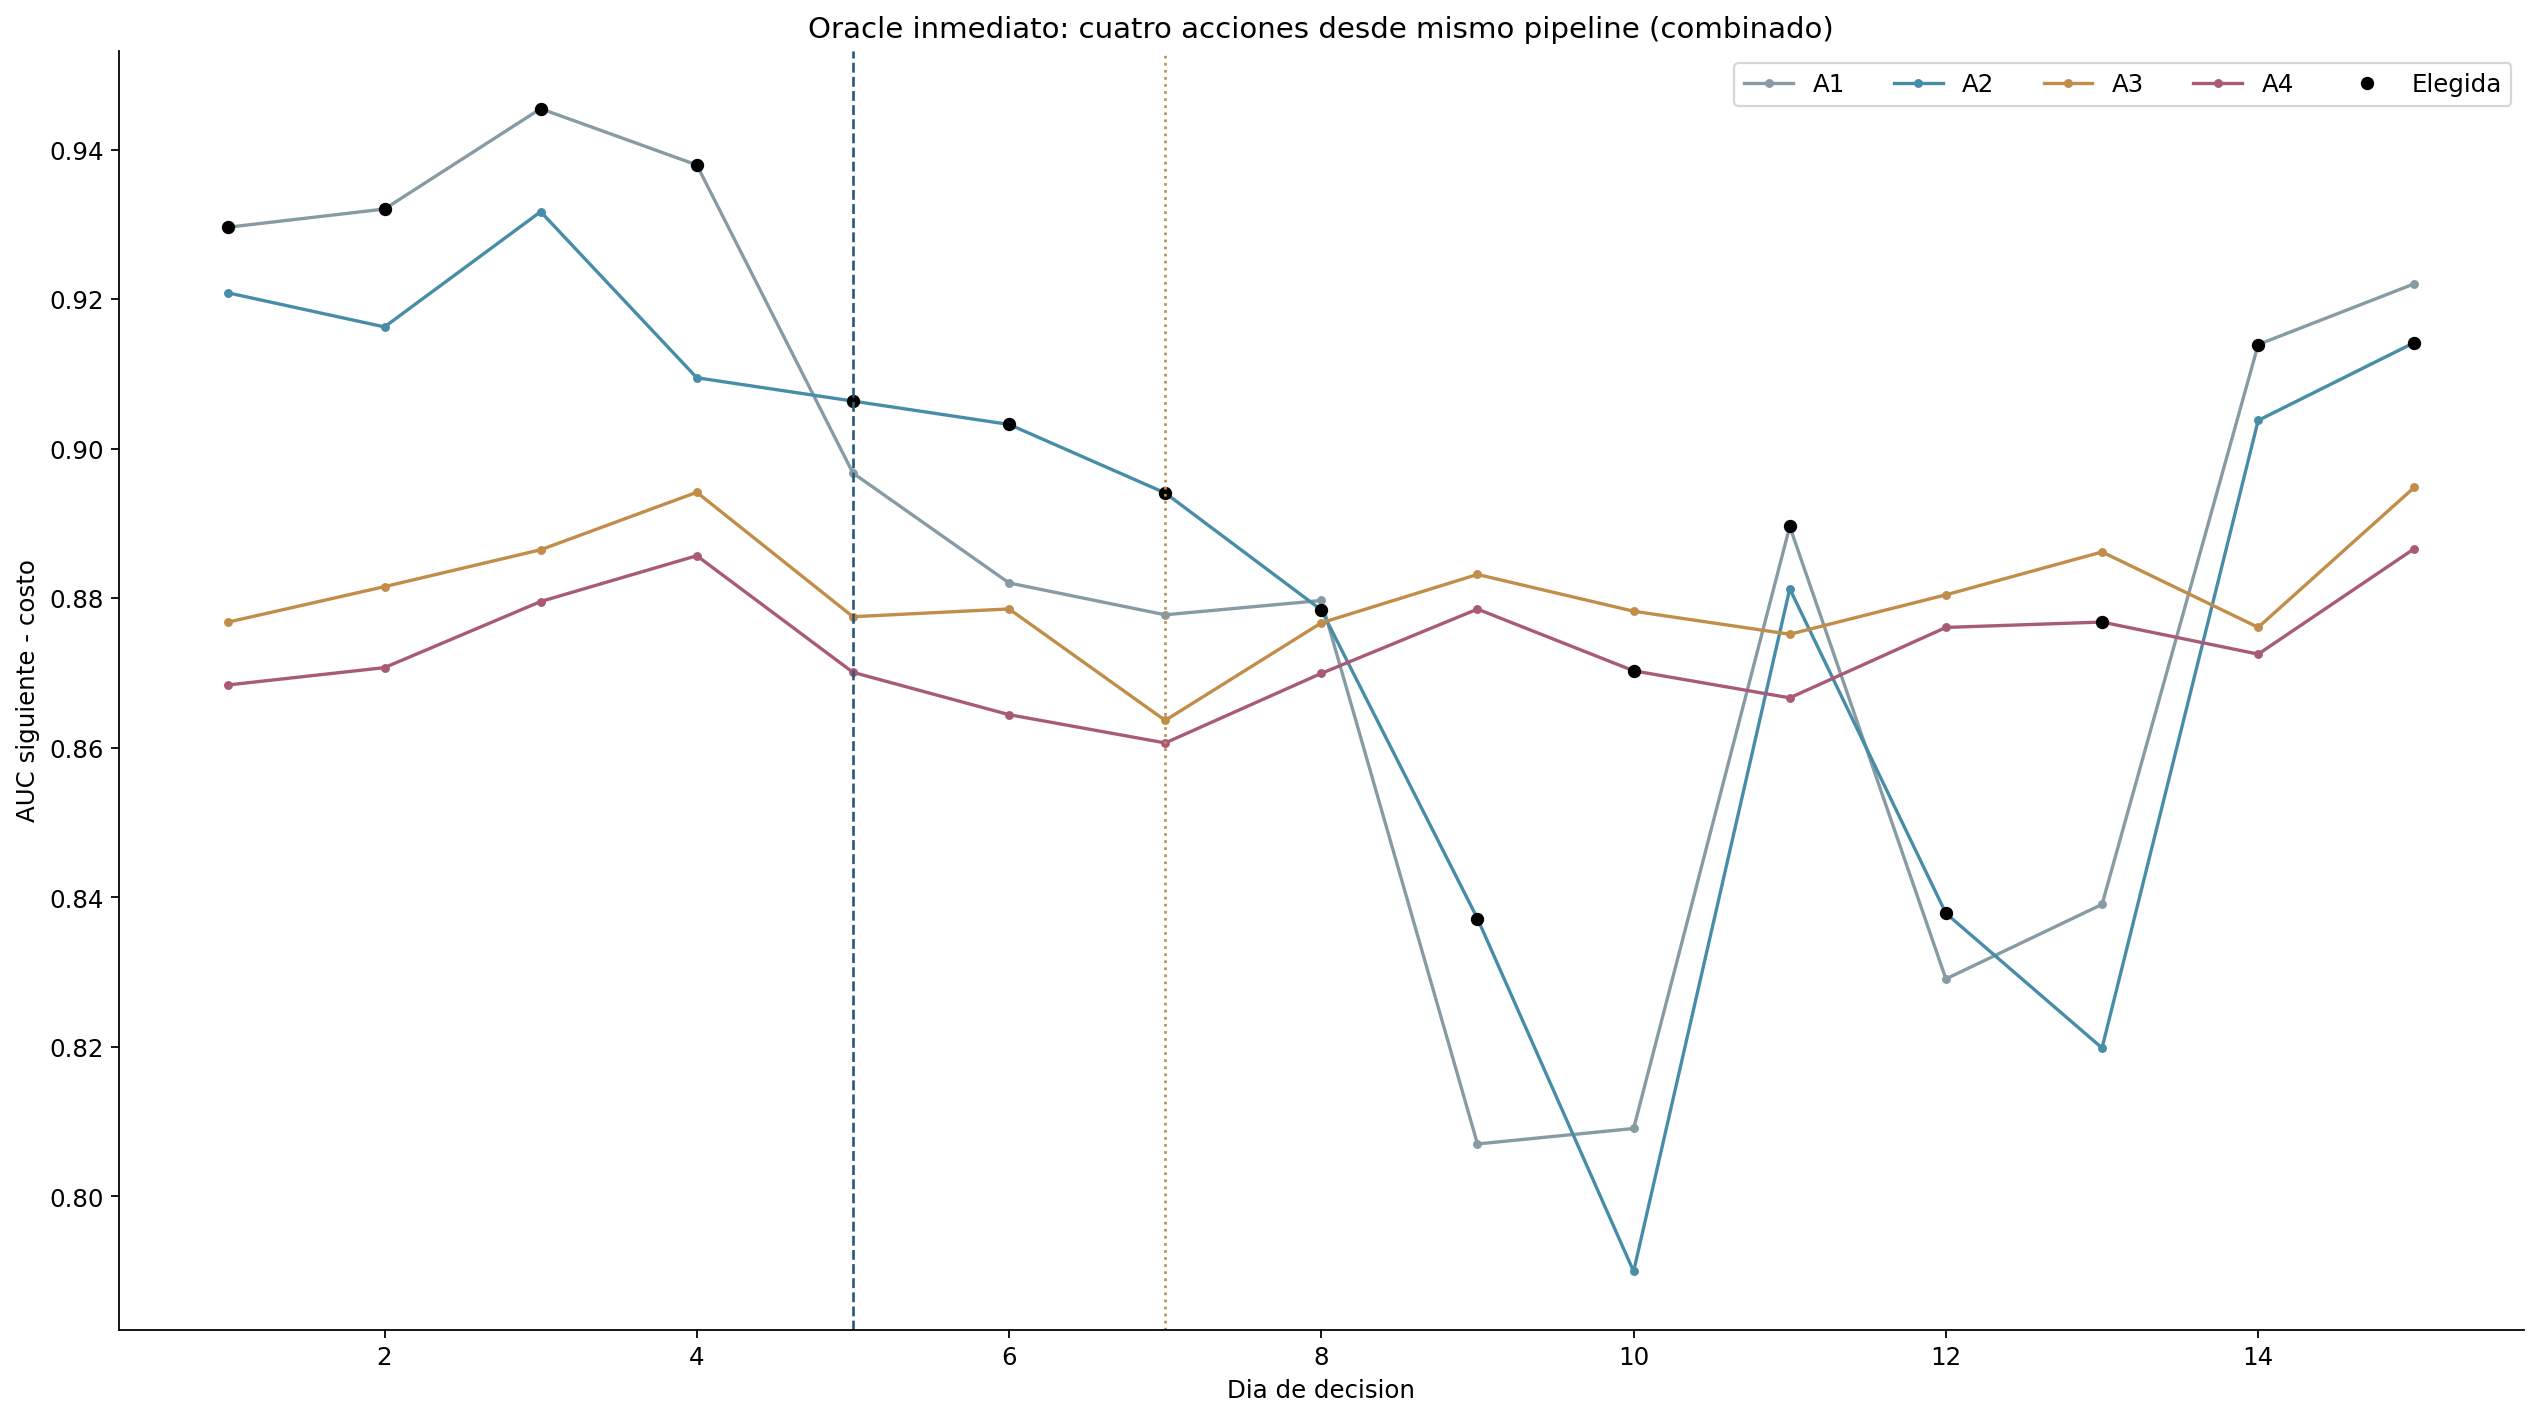
\includegraphics[width=\linewidth,height=0.30\textheight,keepaspectratio]{07a_utilidad_acciones.png}
\vspace{-0.5em}
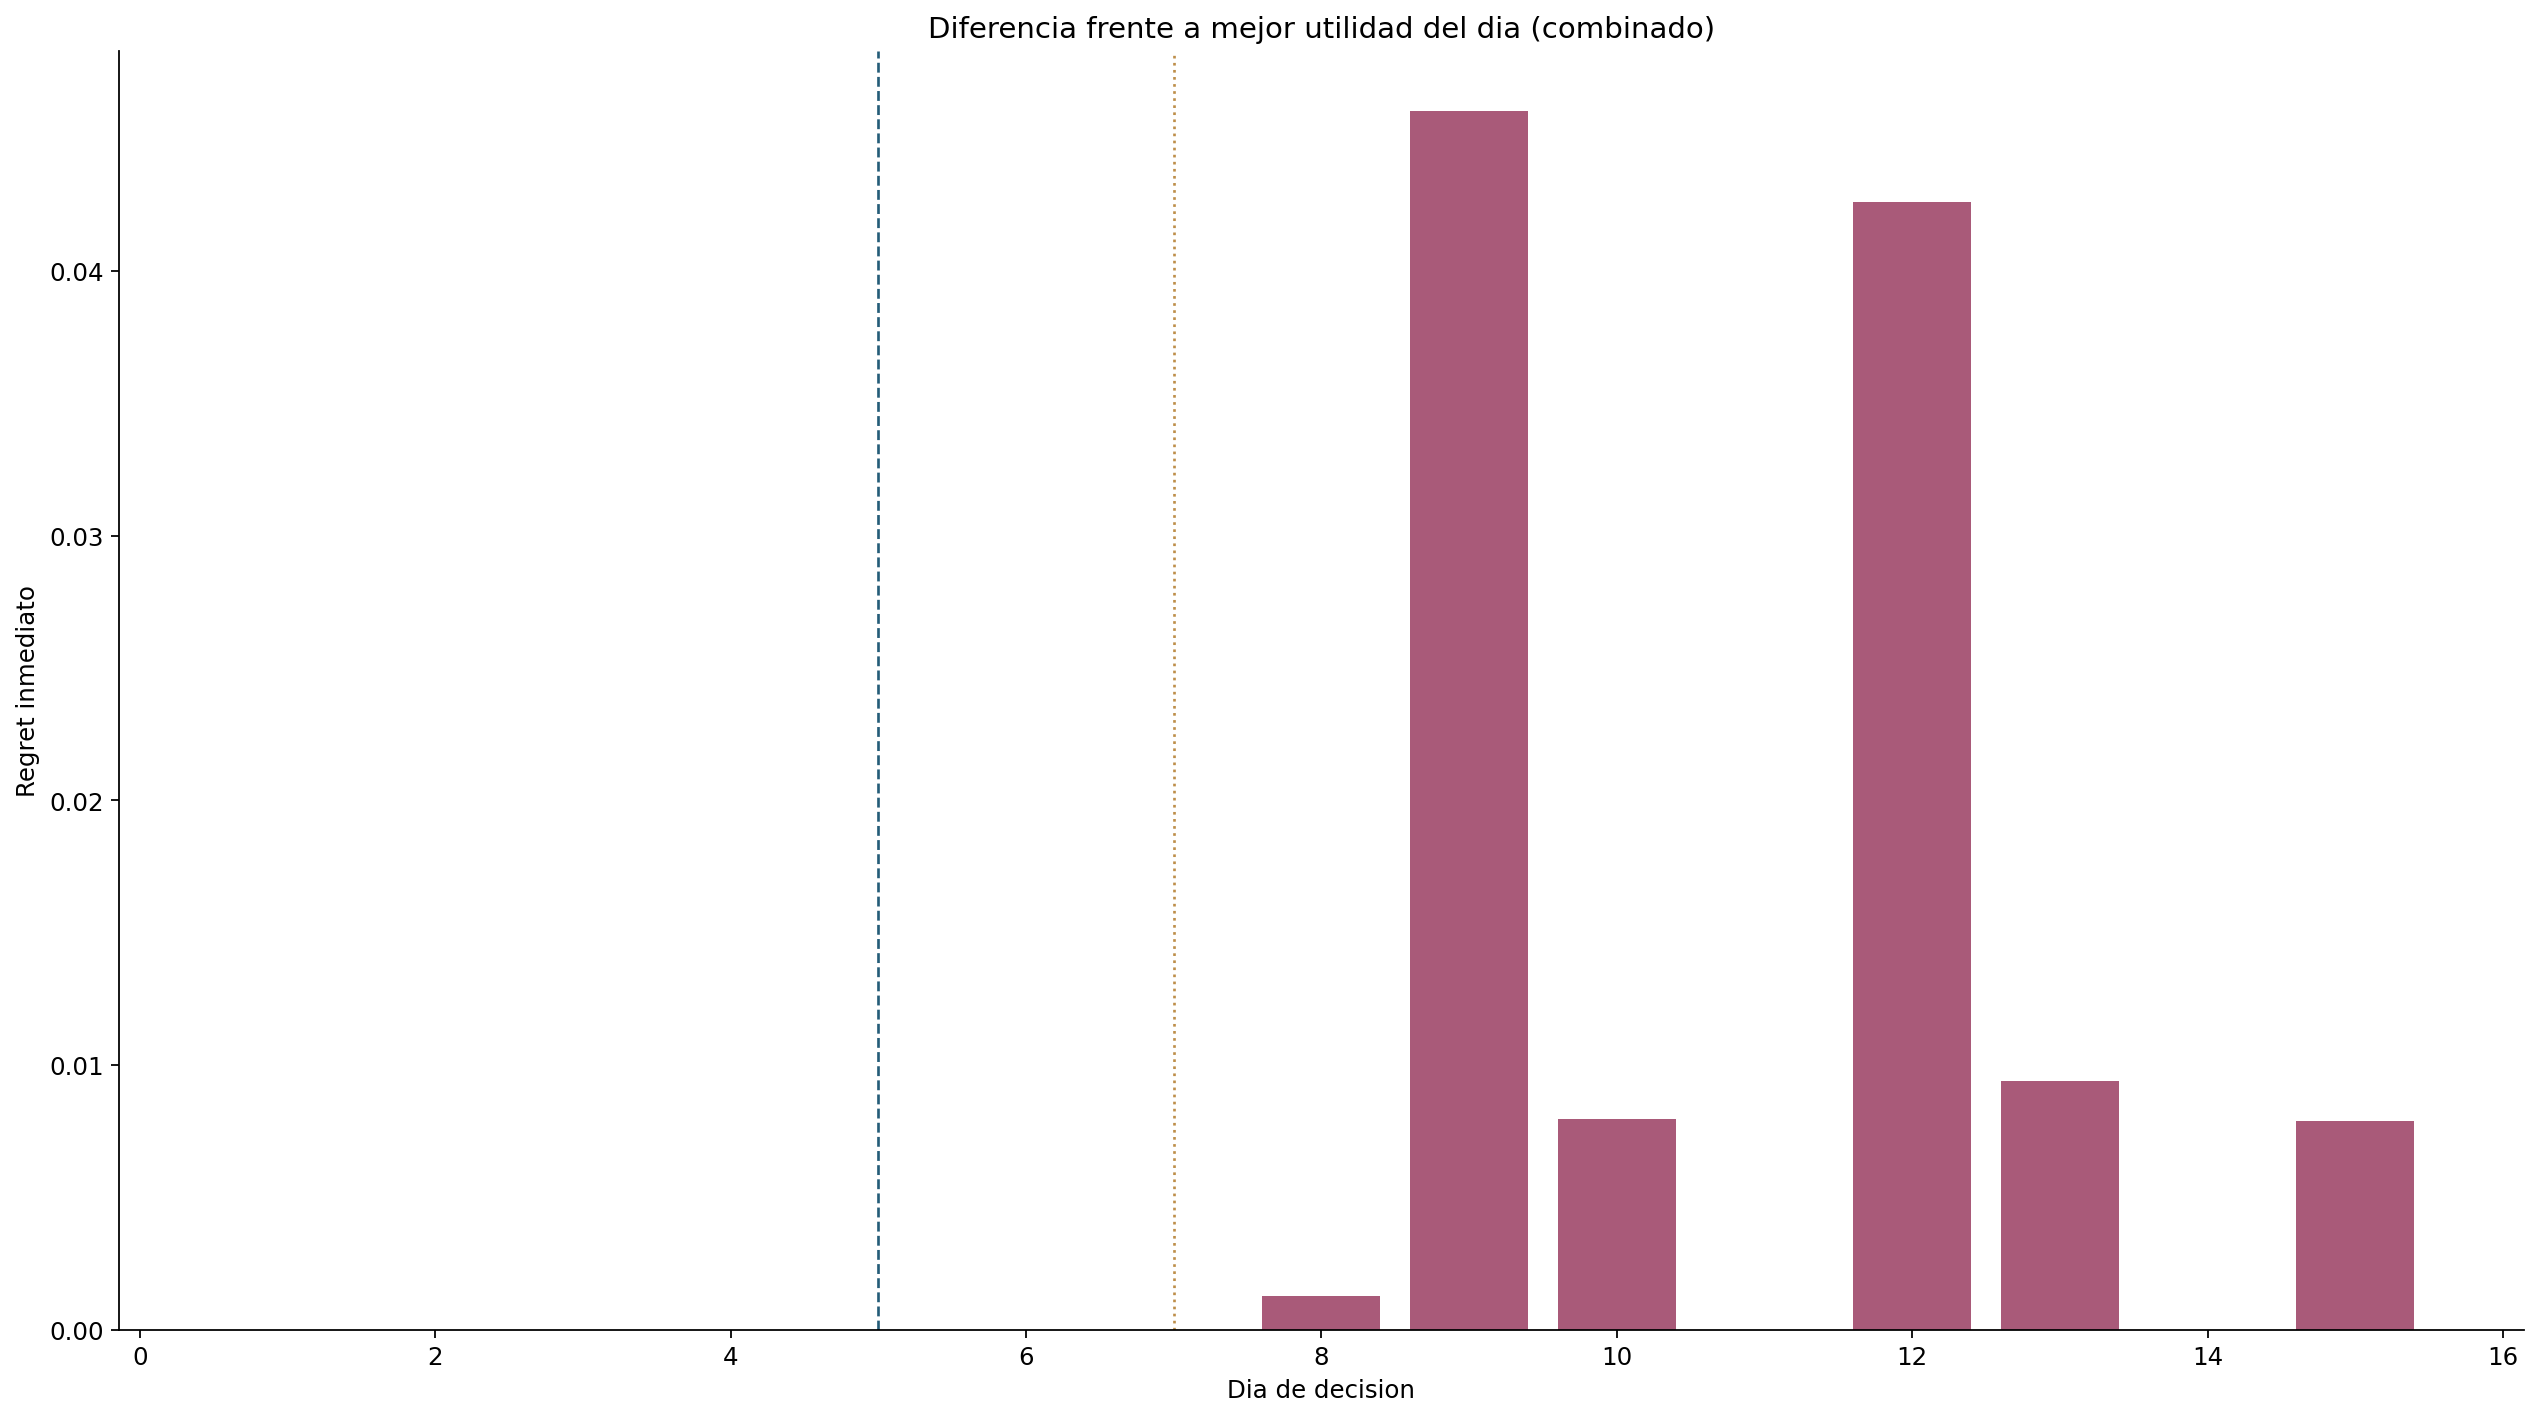
\includegraphics[width=\linewidth,height=0.30\textheight,keepaspectratio]{07b_regret.png}
\end{columns}
{\scriptsize El oracle evalúa la recompensa de un paso para cada acción desde
el pipeline del día; no es una política óptima de horizonte largo.}
\end{frame}

\begin{frame}{Oportunidades donde el oracle inmediato prefiere A3}
\centering
\scriptsize
\begin{tabular}{llrrrr}
\toprule
Escenario & Día & DQN & \(U(A3)\) & \(U\) elegida & Regret \\
\midrule
Concept & 6 & A1 & 0,8783 & 0,8616 & 0,0168 \\
Concept & \textbf{7} & \textbf{A1} & \textbf{0,8759} & \textbf{0,8101} & \textbf{0,0658} \\
Concept & 8 & A3 & 0,8792 & 0,8792 & 0,0000 \\
Concept & 9 & A1 & 0,8855 & 0,8745 & 0,0110 \\
Concept & 14 & A1 & 0,8821 & 0,8564 & 0,0257 \\
Concept & 15 & A1 & 0,8943 & 0,8523 & 0,0420 \\
Combined & \textbf{9} & \textbf{A2} & \textbf{0,8832} & \textbf{0,8371} & \textbf{0,0460} \\
Combined & 10 & A4 & 0,8783 & 0,8703 & 0,0080 \\
Combined & 12 & A2 & 0,8804 & 0,8378 & 0,0426 \\
Combined & \textbf{13} & \textbf{A4} & \textbf{0,8862} & \textbf{0,8768} & \textbf{0,0094} \\
\bottomrule
\end{tabular}

\vspace{0.5em}
\begin{block}{Lectura}
En la prueba, A3 fue oracle inmediato en 10 días y el DQN la eligió una vez.
El regret más alto ocurrió en concept día 7; en combined día 13, elegir A4
quedó a 0,0094 de la utilidad de A3. El oracle es contrafactual de un paso,
no una política óptima de horizonte largo.
\end{block}
\end{frame}

\begin{frame}{Tres decisiones: Q, acción y resultado}
\scriptsize
\setlength{\tabcolsep}{2pt}
\begin{tabular}{p{0.15\textwidth}p{0.24\textwidth}p{0.25\textwidth}p{0.24\textwidth}}
\toprule
 & \textbf{Concept, día 7} & \textbf{Combined, día 9} & \textbf{Combined, día 13} \\
\midrule
Señales & AUC 0,8616; KS 0,0687; PSI 0,0202 & AUC 0,8872; KS 0,2347; PSI 0,1371 & AUC 0,8471; KS 0,2590; PSI 0,1511 \\
\(Q(A1,A2,A3,A4)\) & (1,5023; 1,4581; 1,4218; 1,4546) & (1,1204; 1,1358; 1,0149; 0,8633) & (0,7364; 0,6778; 0,7108; 0,9561) \\
Acción DQN & A1 & A2 & A4 \\
AUC siguiente / reward & 0,8101 / 0,810063 & 0,8457 / 0,837144 & 0,9287 / 0,876802 \\
Oracle A3 / regret & 0,875907 / 0,065844 & 0,883169 / 0,046025 & 0,886176 / 0,009374 \\
\bottomrule
\end{tabular}

\vspace{0.6em}
\begin{itemize}
  \item \textbf{Día 7:} AUC sigue en categoría alta (\(\geq0,85\)) y KS/PSI
        están debajo de sus cortes; las categorías no expresan aún el concept
        activo (\(u=0,45\)), aunque A3 habría elevado la utilidad inmediata.
  \item \textbf{Día 9:} las señales medias de covariate favorecen el valor
        aprendido de A2, pero el oracle de un paso favorece A3.
  \item \textbf{Día 13:} \(Q(A4)\) es claramente mayor; la pérdida frente a A3
        es pequeña y no implica que la política conozca el oracle.
\end{itemize}
\end{frame}

\begin{frame}{Disponibilidad temporal: supuesto del entorno}
\begin{enumerate}
  \item Antes de decidir en el día \(d\), \texttt{BedEnv.\_observe(d)} ejecuta
        \texttt{monitor()} sobre la cohorte eval de ese mismo día y construye
        el estado con KS, PSI y ROC-AUC.
  \item La acción usa la cohorte update del día \(d\); después, la recompensa
        se calcula con ROC-AUC eval del día \(d+1\) menos el costo medido.
  \item \texttt{action\_audit.csv} evalúa offline A1--A4 para medir utilidad y
        regret; esos contrafactuales no se entregan al agente.
\end{enumerate}
\begin{alertblock}{Caveat para interpretación}
El código expone al monitor la etiqueta sintética de la cohorte eval del día
actual antes de la acción; no impone retraso explícito de etiquetas. Es una
hipótesis del simulador, no un mecanismo de aprendizaje con etiquetas
disponibles solo después. Si la tesis asume retraso clínico, el entorno debe
representar ese retraso antes de afirmar que v4 lo respeta.
\end{alertblock}
\end{frame}

\begin{frame}{Por qué falló la estabilidad del 95\%}
\begin{columns}[T]
\column{0.52\textwidth}
\begin{block}{Dos gates distintos}
\begin{itemize}
  \item Variación relativa del retorno en los últimos cinco checkpoints:
        \textbf{1,47\%}; pasa el límite \(\leq 5\%\).
  \item Estabilidad exacta: proporción de acciones idénticas entre los dos
        últimos checkpoints de validación: \textbf{85\%}; no pasa
        \(\geq 95\%\).
  \item La tolerancia de empate Q de 0,005 también dio 85\%: esa tolerancia no
        explicó las diferencias de acción.
\end{itemize}
\end{block}
\column{0.48\textwidth}
\begin{block}{Diagnóstico observable}
\begin{itemize}
  \item La evaluación usa 60 situaciones (4 escenarios \(\times\) 15 días):
        85\% equivale a unas 51 coincidencias y 9 cambios entre checkpoints.
  \item El acuerdo fue volátil en el tramo final: 35\% en ep. 960,
        38\% en ep. 970, 87\% en ep. 980 y 85\% en ep. 1000.
  \item Se agotaron los 1000 episodios; no hubo evidencia de convergencia
        estable al cierre.
\end{itemize}
\end{block}
\end{columns}
\vspace{0.2em}
\begin{alertblock}{Interpretación}
El retorno puede variar poco aunque algunas acciones cambien, por compensación
entre días/escenarios. La métrica de retorno no certifica que la regla de
decisión se haya estabilizado.
\end{alertblock}
\end{frame}

\begin{frame}{Qué sugiere la trayectoria de estabilidad}
\begin{columns}[T]
\column{0.49\textwidth}
\begin{block}{Evidencia directa}
\begin{itemize}
  \item En checkpoints finales, el acuerdo fue 35\% (ep. 960), 38\% (970),
        87\% (980), 83\% (990) y 85\% (1000).
  \item Ningún acuerdo de checkpoint registrado alcanzó 95\%.
  \item El retorno cambió poco en conjunto, pero la identidad de las acciones
        no se asentó.
\end{itemize}
\end{block}
\column{0.51\textwidth}
\begin{block}{Explicaciones que deben probarse}
\begin{itemize}
  \item La observación usa categorías discretas de KS/PSI/AUC y tres días de
        historial: puede ocultar cambios graduales o diferencias entre
        situaciones.
  \item El agente aprende sobre escenarios, inicios y velocidades diversos;
        la mezcla puede producir valores \(Q\) cambiantes entre políticas con
        retornos parecidos.
  \item El concept drift demanda señal supervisada; el DQN también reaccionó
        tarde y eligió poco A3 en prueba.
\end{itemize}
\end{block}
\end{columns}
\vspace{0.2em}
{\footnotesize Las dos primeras viñetas de la derecha son hipótesis
metodológicas, no causas demostradas por una sola corrida. Se deben contrastar
con márgenes Q, acuerdos por escenario y varias semillas.}
\end{frame}

\begin{frame}{Una limitación del gate que debe corregirse}
\begin{itemize}
  \item El checkpoint seleccionado para reportar la política fue el
        \textbf{episodio 940}, elegido por media móvil de tres validaciones.
  \item Sin embargo, el gate final compara las acciones de los
        \textbf{dos últimos checkpoints} (ep. 990 y 1000), no la estabilidad
        alrededor del checkpoint seleccionado.
  \item Por tanto, 85\% describe la estabilidad al final del entrenamiento,
        pero no mide directamente cuánto cambia la política seleccionada en
        ep. 940 respecto a sus vecinos.
  \item Esta desalineación no invalida que el gate actual falló; sí limita la
        interpretación del fallo como inestabilidad del checkpoint que se
        reportó en prueba.
\end{itemize}
\vspace{0.4em}
\begin{block}{Conclusión metodológica}
Definir primero qué política se desplegará y evaluar estabilidad sobre esa
política y checkpoints vecinos. No basta con cambiar el umbral o con aumentar
episodios.
\end{block}
\end{frame}

\begin{frame}{Plan para perseguir el 95\% sin sobreajustar}
\begin{enumerate}
  \item \textbf{Alinear selección y gate:} congelar una validación; elegir
        checkpoint con la regla declarada y medir acuerdo antes/después de ese
        checkpoint, además de retorno.
  \item \textbf{Exigir persistencia:} registrar acuerdo por escenario y
        requerir que el gate se mantenga en varios checkpoints consecutivos,
        no solo en un par aislado.
  \item \textbf{Diagnosticar cambios:} reportar matriz de transición de
        acciones y margen entre los dos mayores valores \(Q\); separar cambios
        en estable, covariate, concept y combinado.
  \item \textbf{Mejorar señal y cobertura de entrenamiento:} evaluar AUC
        continua y su tendencia, validez/atraso de etiquetas y tiempo desde la
        última acción; variar inicios y velocidades de drift en B-train.
  \item \textbf{Ajustar solo en train/validación:} probar exploración,
        tasa de aprendizaje, replay y actualizaciones del target. No asumir
        que más episodios resolverán la inestabilidad: v4 llegó al máximo.
  \item \textbf{Repetir con varias semillas} y reservar B-test intacto para la
        evaluación final. Mantener el 95\% como gate preregistrado; no bajar
        el umbral para declarar éxito.
\end{enumerate}
\end{frame}

\begin{frame}{Cómo cuantificar la meta}
\begin{block}{Si se mantienen 60 decisiones de validación}
Para cumplir \(95\%\) se requieren al menos \(57/60\) acciones coincidentes.
El resultado actual es aproximadamente \(51/60\); hay que reducir al menos
seis desacuerdos en ese conjunto, sin degradar utilidad ni variar la definición
del gate.
\end{block}
\begin{itemize}
  \item No tratar \(57/60\) como certificado estadístico independiente: las
        decisiones comparten episodios y estados; repetir semillas y escenarios
        mide robustez mejor que ampliar solo la misma secuencia.
  \item Reportar junto al porcentaje: total de estados, acuerdo por escenario,
        acciones que cambian, diferencias de \(Q\), retorno y regret.
  \item Un criterio de equivalencia por regret puede complementar el acuerdo
        exacto, pero debe reportarse por separado; no sustituye el gate del
        95\% solicitado.
\end{itemize}
\end{frame}

\begin{frame}{Conclusiones y trazabilidad}
\begin{itemize}
  \item La utilidad depende del régimen: A2 es la actualización selectiva más
        eficiente para covariate drift; A3 recupera ante concept drift; A1
        evita intervenciones perjudiciales en el escenario estable.
  \item v4 no superó estabilidad porque el acuerdo exacto final fue 85\%, pese
        a que la variación del retorno fue baja. La política cambió con
        frecuencia al final del entrenamiento.
  \item La selección en ep. 940 y el gate en ep. 990--1000 no están alineados;
        corregir esa medición es el primer paso antes de nuevas corridas.
  \item El benchmark usa objetivo sintético, una semilla y costos de tiempo
        dependientes del entorno: interpretar como prueba de método,
        no como evidencia clínica o económica.
\end{itemize}
\vspace{0.4em}
\footnotesize
\textbf{Fuentes de resultados:} \texttt{run\_summary.json},
\texttt{policy\_comparison.csv}, \texttt{action\_audit.csv} y
\texttt{training\_history.csv}, en
\texttt{kaggle/dqn-dummy/v4/outputs/}. Diseño: \texttt{plan/dqn-dummy-v4.md}.
\end{frame}

\begin{frame}[allowframebreaks]{Referencias metodológicas}
\footnotesize
\begin{thebibliography}{9}
\bibitem{reyna2020sepsis}
M. A. Reyna et al., ``Early Prediction of Sepsis From Clinical Data: The
PhysioNet/Computing in Cardiology Challenge 2019,''
\emph{Critical Care Medicine}, vol. 48, no. 2, pp. 210--217, 2020,
doi: 10.1097/CCM.0000000000004145.

\bibitem{mnih2015dqn}
V. Mnih et al., ``Human-level control through deep reinforcement learning,''
\emph{Nature}, vol. 518, pp. 529--533, 2015,
doi: 10.1038/nature14236.

\bibitem{chen2016xgboost}
T. Chen and C. Guestrin, ``XGBoost: A Scalable Tree Boosting System,''
in \emph{Proceedings of the 22nd ACM SIGKDD International Conference on
Knowledge Discovery and Data Mining}, 2016, pp. 785--794,
doi: 10.1145/2939672.2939785.

\bibitem{doubleq}
H. van Hasselt, A. Guez, and D. Silver, ``Deep Reinforcement Learning with
Double Q-learning,'' in \emph{Proceedings of the AAAI Conference on
Artificial Intelligence}, vol. 30, no. 1, 2016.

\bibitem{data_caveat}
El target \texttt{y\_dummy}, el calendario de drift y el replay son
construcciones de la demostración v4; no forman parte de PhysioNet ni describen
la progresión clínica de sepsis.
\end{thebibliography}
\end{frame}

\end{document}
